\begin{figure}[h!]
    \centering
    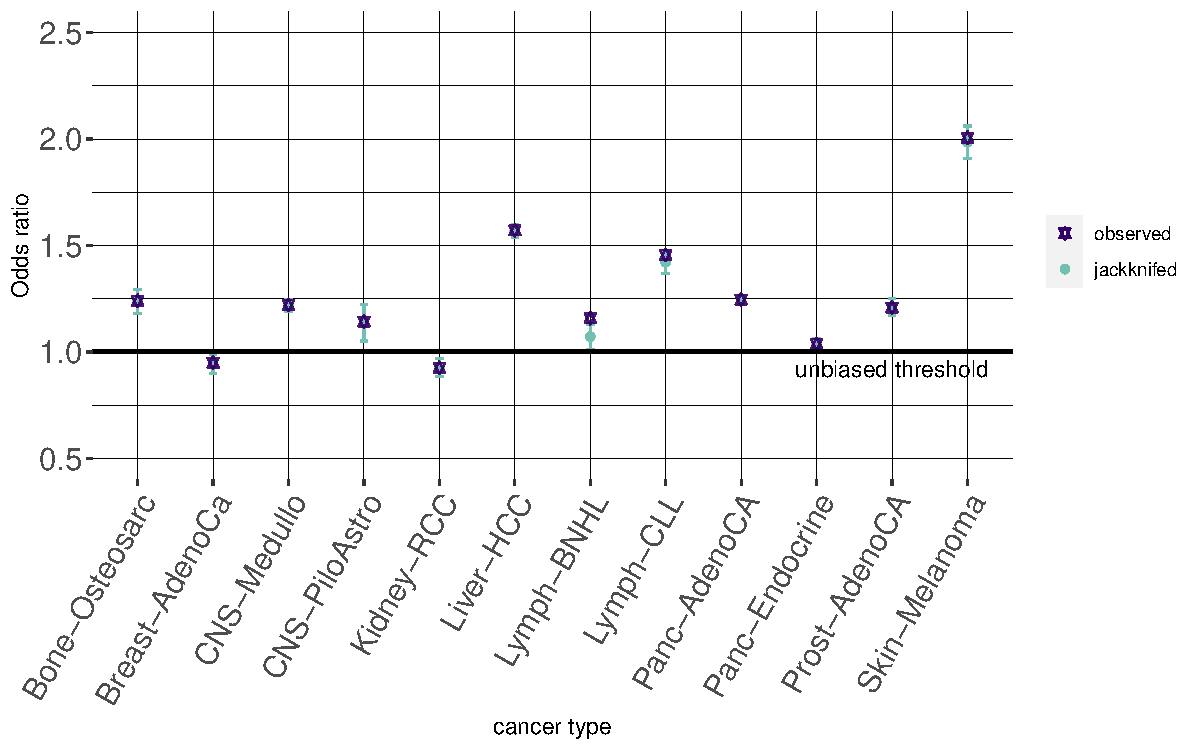
\includegraphics[scale=0.75]{graphics/jackknife_OR.pdf}
\caption{}
    % \caption{\textbf{Mutations tended to occur in closed chromatin regions according to the odds ratio ($OR$) statistic}. $OR>1$ indicates a bias towards towards closed regions, and $OR<1$ indicates the opposite. Error bars are the standard errors of the jackknifed sample. The green circles are the means of the jackknifed pseudo-values. The purple stars are the observed $OR$.}
    \label{fig:or_jackknifed}
\end{figure}
